\chapter{Experiment}
\label{ch:exp}
In the experiment an FTB-300 ``Universal Test System''by EXFO was used to characterize optical links and an optical network. To perform the OTDR measurements an in the FTB-300 integrated FTB-7323B was used. In the first experimets a model standard link is examined. The OTDR is connected to a spool of fiber by a patchcord. Another patchcord connects the end of the fiber to another spool of fiber. The end of the fiber is terminated by an open APC connector. 

Figure \ref{fig:1_line} shows the OTDR measurement for the setup. The measurement complete measurement settings can be found in the appendix.
At the distance near $x$~=~0 there is a large reflection caused by the OTDR. The range from $ 0$~km$~ < x < 10$~km shows the first 10~km spool of fiber. The slope is caused by Rayleigh scattering (cf. {\ref{loss}}). At $x = 10~$km a step in the measurement can be observed. At this location the spool of fiber is connected to another spool using a patchcord and APC connectors. This connectors lead to losses. 
The range from $10$~km~$ < x < 20$
~km shows the second spool of fiber. At $x = 20$~km the signal drops significantly at the end of the line.


\begin{figure}[h]%
\centering
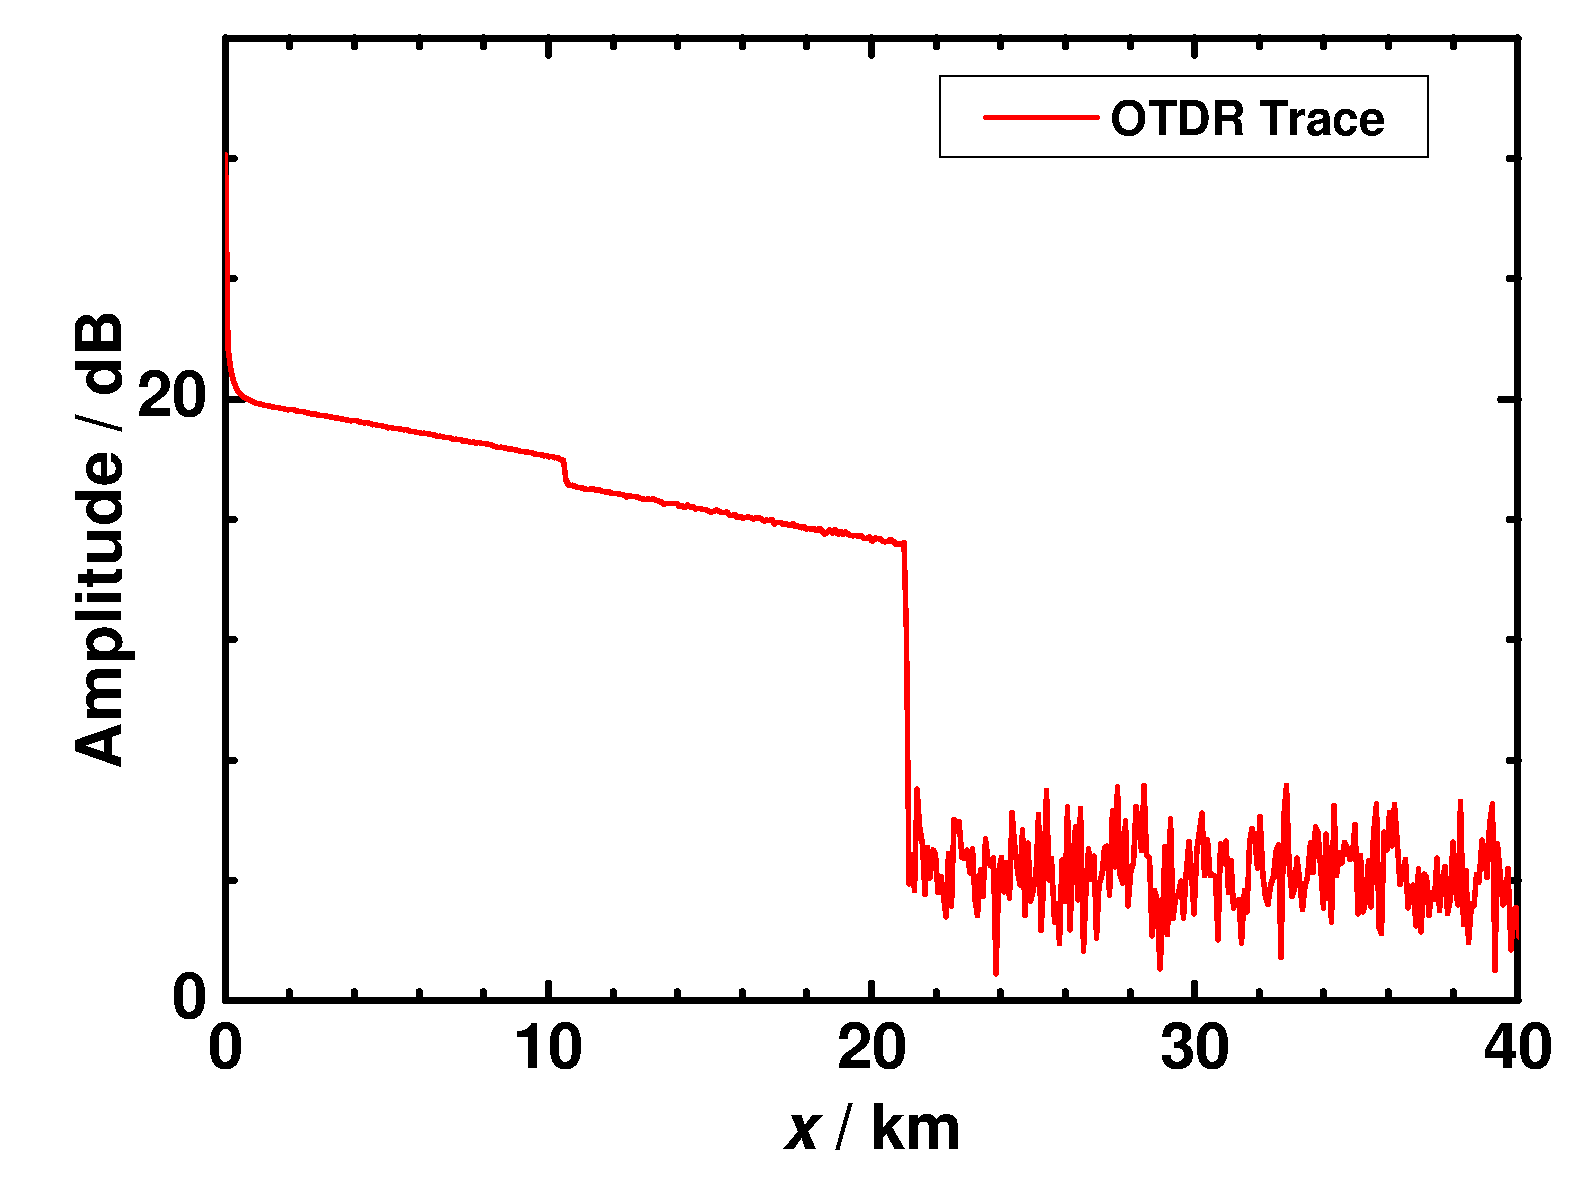
\includegraphics[width=.6\columnwidth]{grafiken/1_line.pdf}%
\caption{Backscattered signal of the setup. (TRACE008)}%
\label{fig:1_line}%
\end{figure}
\newpage

\section{Effects of OTDR measurement parameters on the measurements}
In the first task the effects of the OTDR measurement parameters on the measurement was analyzed. 
The following parameters were set:
\begin{itemize}
	\item \textbf{Wavelength} - The FTB-300 is able to measure with two different wavelength. At the zero dispersion wavelength $\lambda ~=~1310~$nm  of silica based optical fibers and at $\lambda~=~1550$~nm the minimum-loss window for silica based optical fibres.
	\item \textbf{Pulse Width} - The pulse width determines for one thing the resolution of the OTDR (cf. \ref{sec:resolution}), for another thing the maximum measurement distance. 
	\item \textbf{Integration Time} - The OTDR does several measurements and integrates over the preset time to reduce noise. 
\end{itemize}

To determine the effects of the pulse length on the measurement several different length were tested. To demonstrate the effects traces of 5 different pulse length are put into one graph (eg. \ref{fig:1_time}). The integration time for all traces was 30~s. The complete data can be found in the appendix.

Comparing the different traces shown in figure \ref{fig:1_time} leads to the fact, that longer pulses in time lead to an higher signal amplitude. This is obvious since this pulse carries the most energy compared to the other pulses. 
The lowest signal amplitude therefore hast the smallest measured pulse, with a pulse width of $t\i{pulse}$~=~10~ns. But due to the low energy the small pulse carries the signal of short pulses shows higher influence of noise than the longer pulses. 


\begin{figure}[h]%
\centering
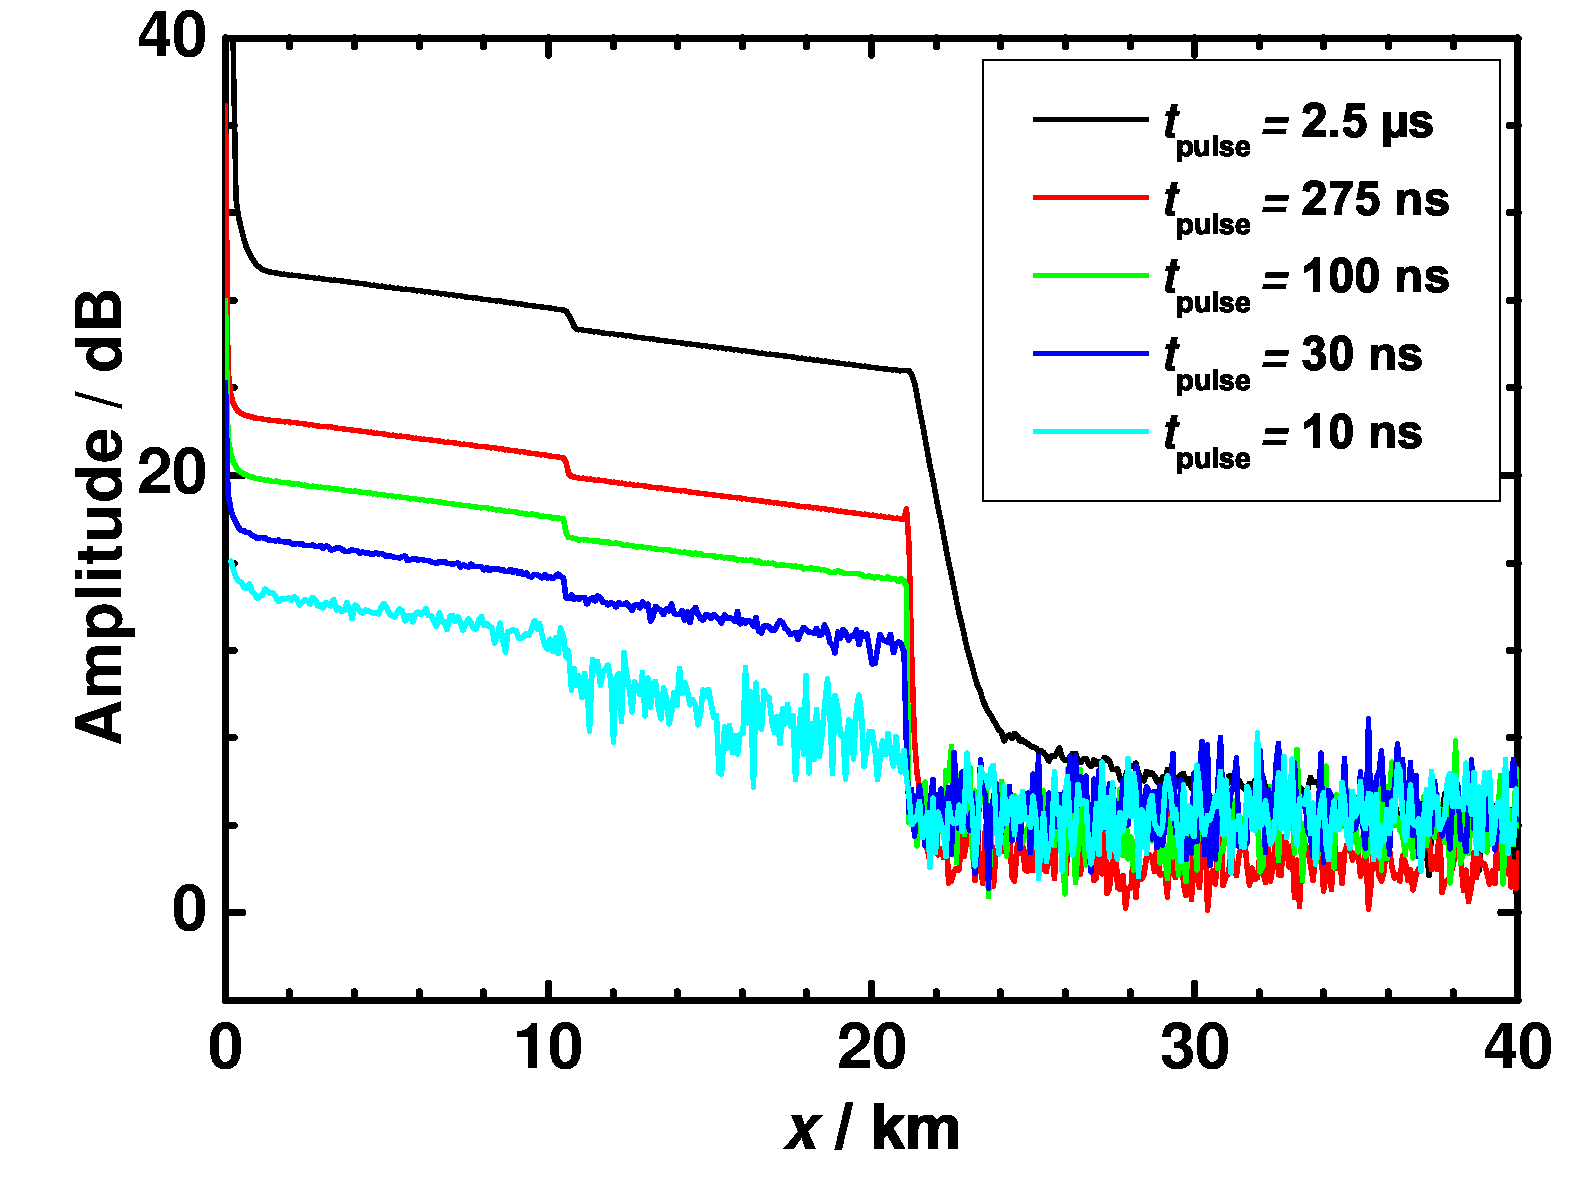
\includegraphics[width=.6\columnwidth]{grafiken/1_time.pdf}%
\caption{Backscattered signal for different pulse widths. (2.5 $\upmu$s: TRACE000, 275 ns: TRACE001, 100~ns: TRACE002, 30~ns: TRACE003, 10~ns: TRACE004). All measurements with an integration time of 30~s.}%
\label{fig:1_time}%
\end{figure}
\newpage

At a distance of $x$~$\approx$~20~km the end of the line can be observed.
The trace of the long pulse shows a large dead zone compared to the other. The signal needs up to 5~km to reach the low signal value the other traces show at this distance. 


To achieve the best performance a compromise between a heigh resolution (small pulse) and a low noise level (large pulse) needs to be found.

To reduce the noise level of the small pulses the integration time can be enlarged.therefore a pulse lenght of 100~ns was selected and the integration time was varied from 30~s to 2~min. 


\begin{figure}[t]%
\centering
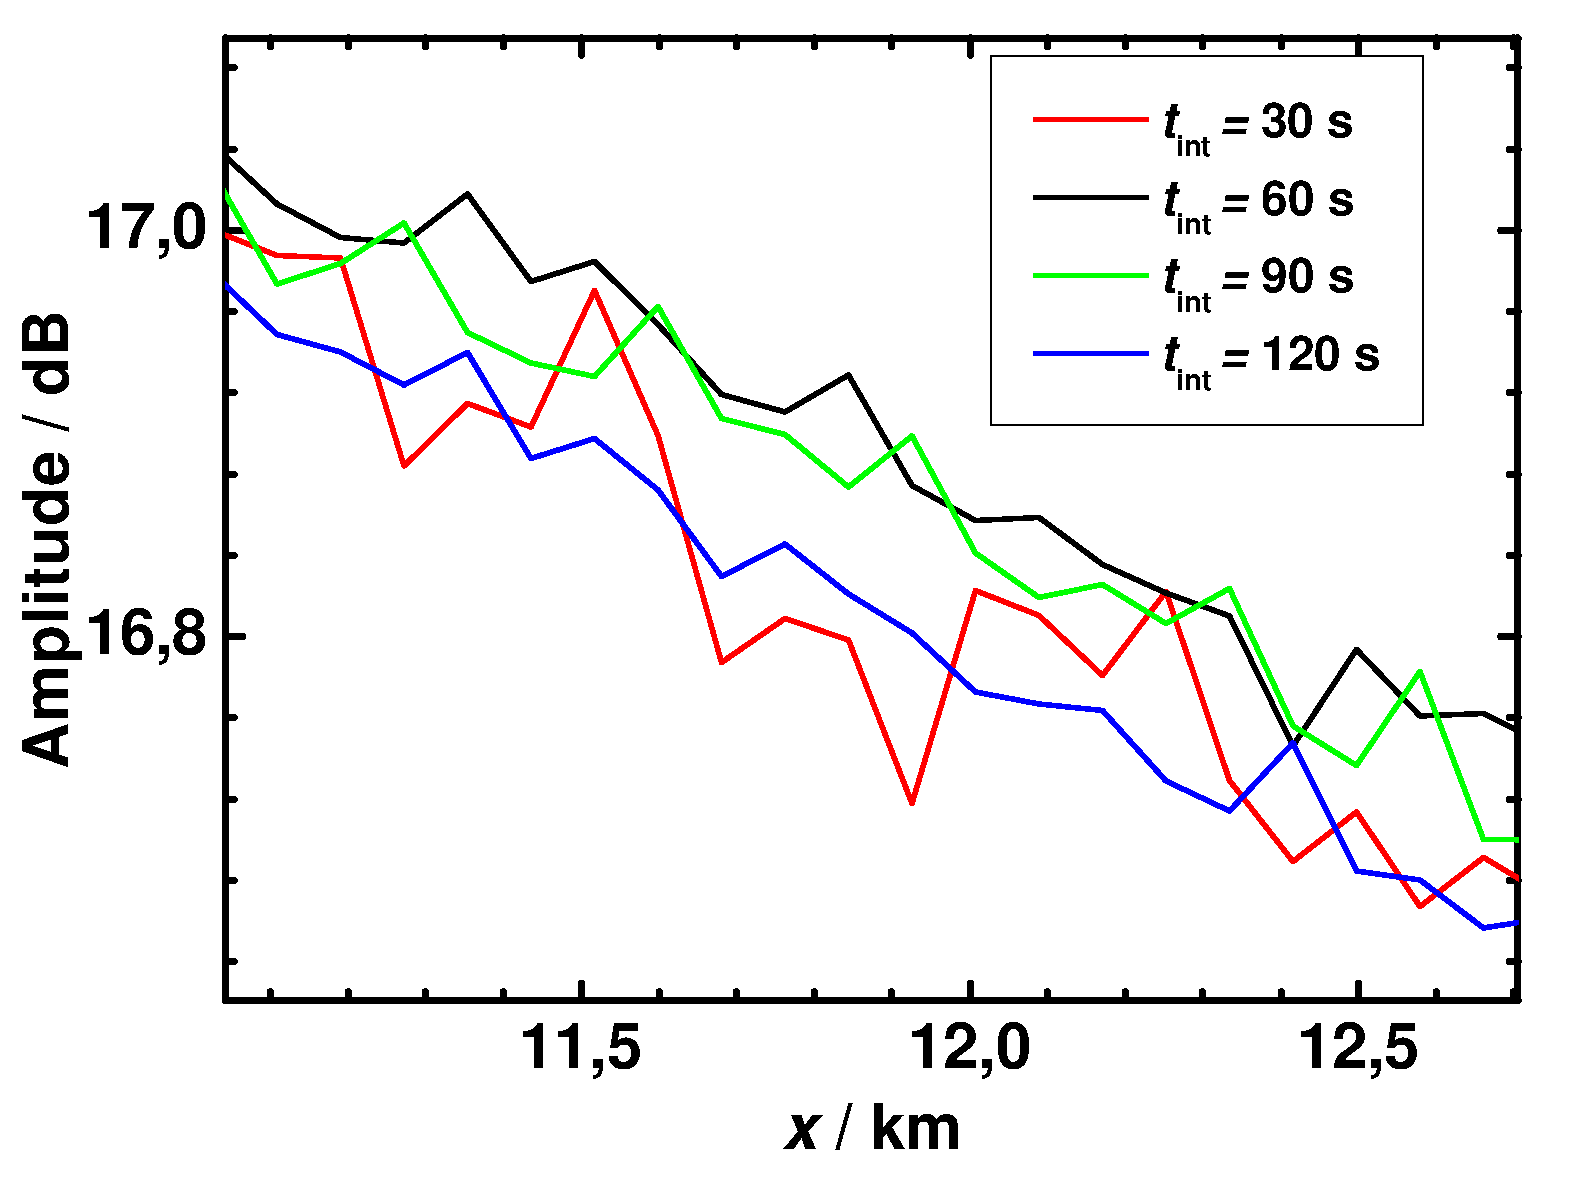
\includegraphics[width=.6\columnwidth]{grafiken/1_integration.pdf}%
\caption{Backscattered signal for different integration times. (30 s: TRACE009, 60 s: TRACE008, 90~s: TRACE010, 120~s: TRACE011). All measurements with a pulse width of 100~ns.}%
\label{fig:integration}%
\end{figure}

Figure \ref{fig:integration} shows a detail of the traces with a 100~ns pulse width for different integration times. The complete data can be found in the appendix.

Changing the integration time leads to a variation of the noise level. An integration time of 30~s leads to an variation of $\sim$0.1~dB. A longer integration time results in a lower variation of the signal. 
Doubling the integration time to 60~s gives an variation of the signal of $\sim$0.02~dB. Increasing the integration time even further gives nearly no improvement of the signal variation but leads to long measurement times.
For this reason the the integration time was set to 1 minute and since the trace with a pulse with 100~ns pulse width shows low noise and a good resolution those parameters were chosen for the following measurements.

Last the influence of the wavelength was examined. Figure \ref{fig:1_lambda} shows the OTDR measurement for the two different wavelenght. Both traces were measured with a pulse width of 100~ns and an integration time of 1 minute. The complete data can be found in the appendix.

\begin{figure}%
\centering
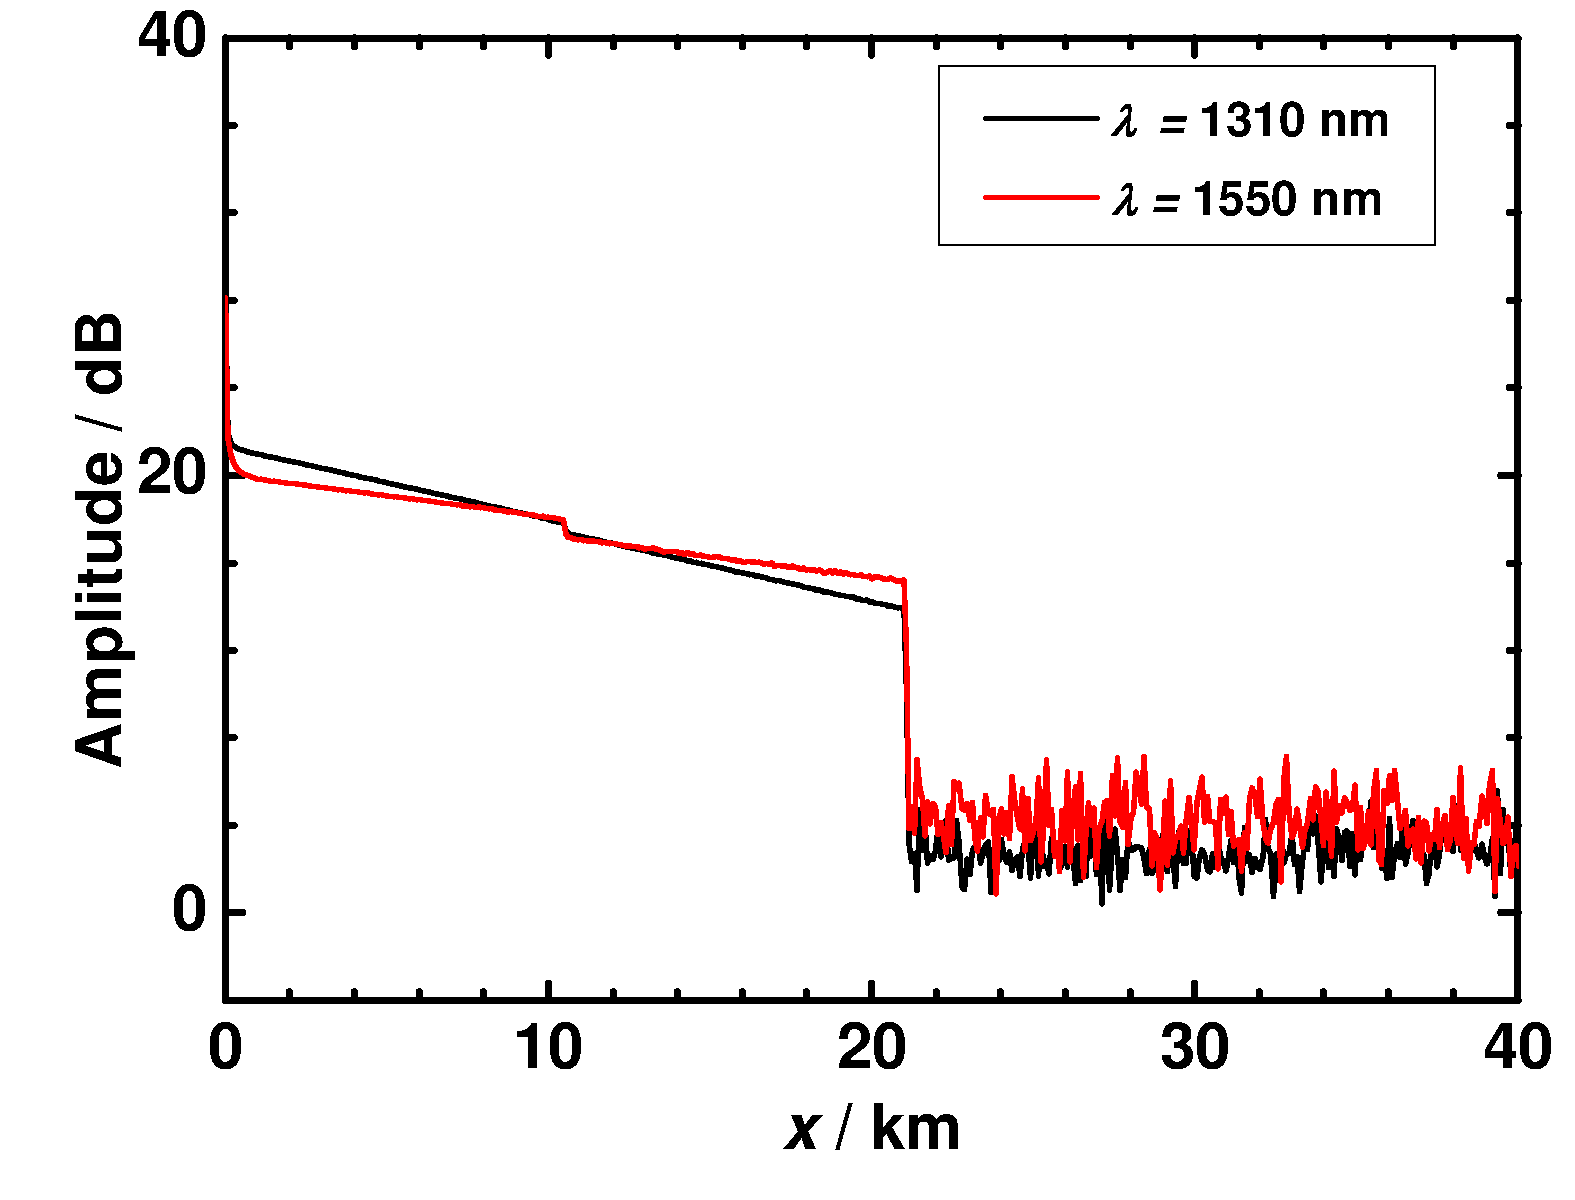
\includegraphics[width=.6\columnwidth]{grafiken/1_lambda.pdf}%
\caption{Backscattered signal for different wavelengths. (1310~nm: TRACE012, 1550~nm: TRACE008). Both measurements with a pulse width of 100~ns and an integration time of 1 minute.}%
\label{fig:1_lambda}%
\end{figure}

Using the EXFO OTDR FTB-7000 software the attenuation of the optical fiber at both wavelengths can be measured at the slopes of the trace. Table \ref{tab:1_daempfung} shows the attenuation at both wavelenghts.

\begin{table}[h]%
\centering
\caption{Attenuation of the optical fiber}
 
\begin{tabular}{cc}

\toprule

$\lambda$	& Attenuation\\
\midrule
1310 nm & 0.34 dB / km\\
1550 nm& 0.19 dB / km\\
\bottomrule 
\end{tabular}
\label{tab:1_daempfung}
\end{table}

The fiber shows a larger attenuation at $\lambda~=~$1310~nm than at $\lambda~=~1550$~nm. This behaviour is expected since the minimum-loss window for silica based optical fibers is at this wavelength. 



\section{Effects of a loose connector on the measurements}

\begin{figure}%
\centering
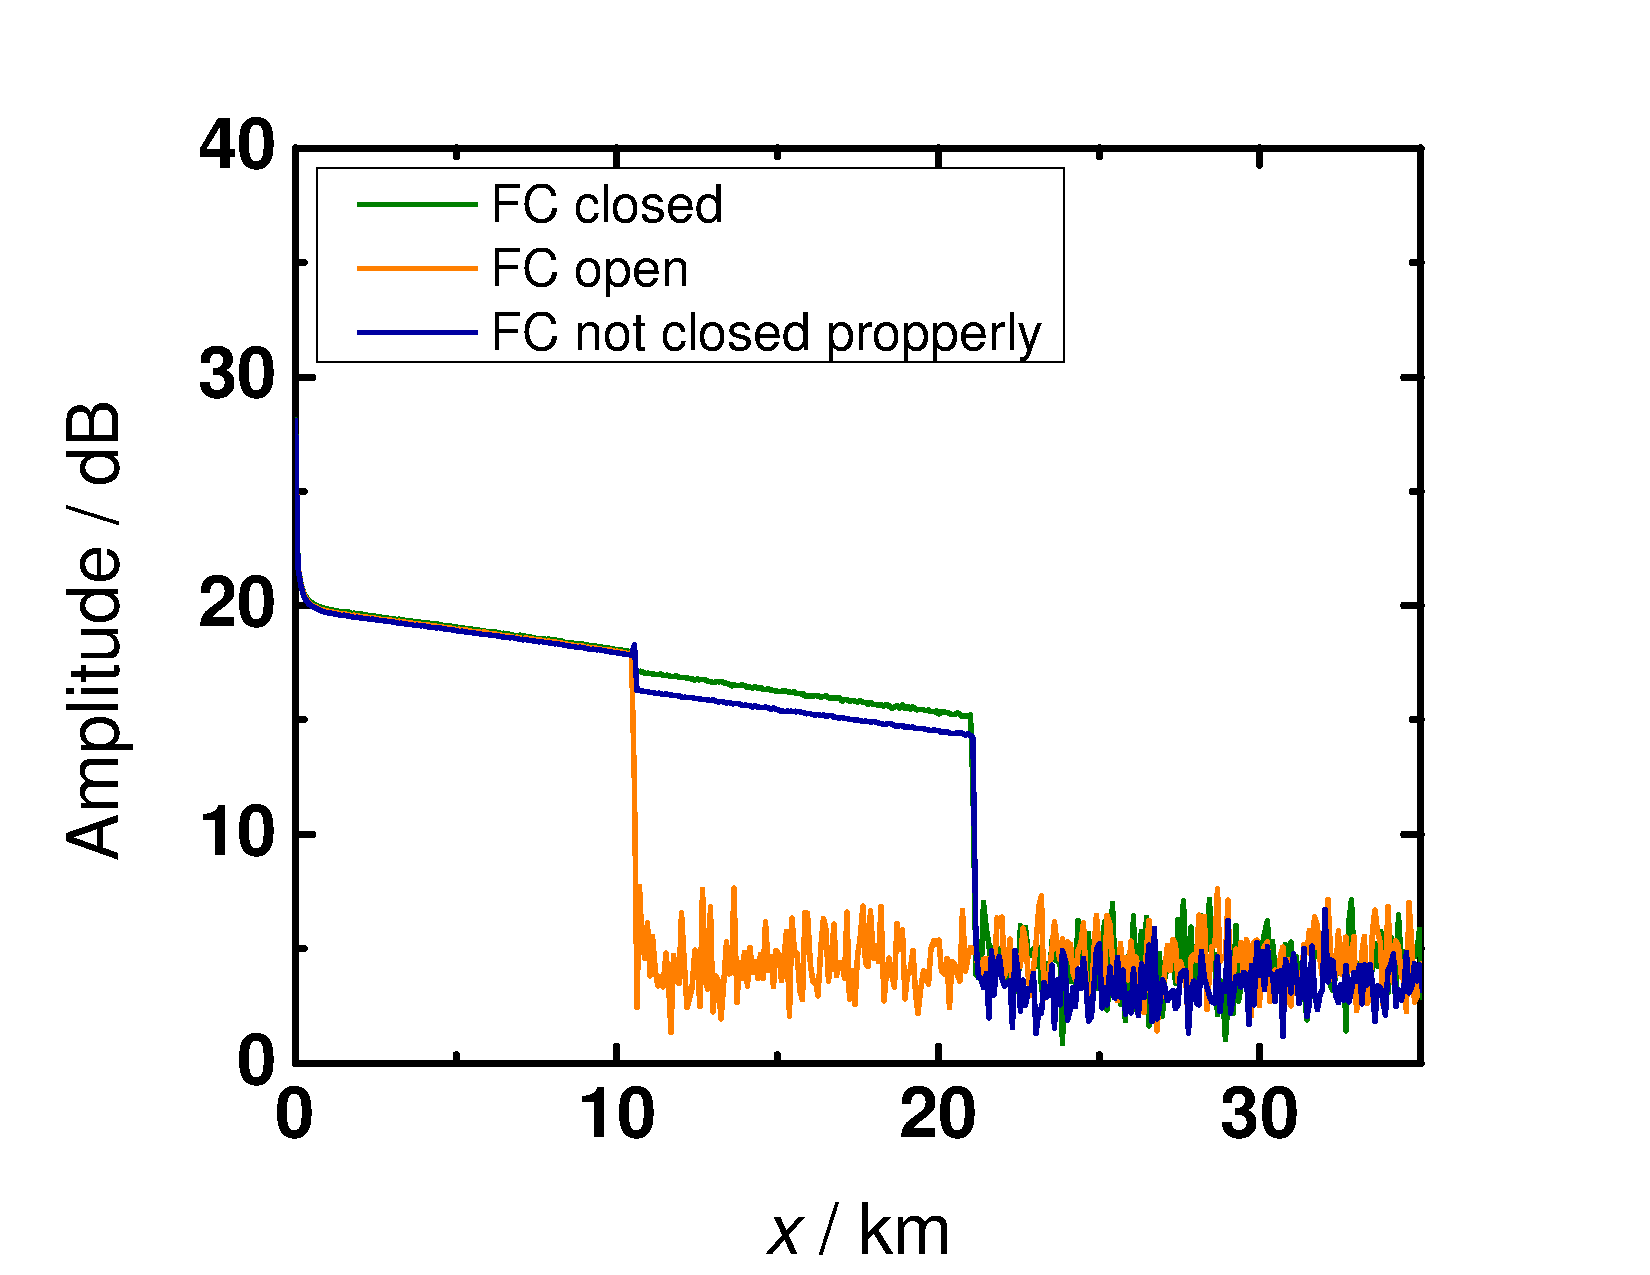
\includegraphics[width=.8\columnwidth]{grafiken/Connector.pdf}%
\caption{}%
\label{fig:connector}%
\end{figure}

In this experiment a connector at the patchcord between the two fibers is loosend. The measurements for this are shown in figure \ref{fig:connector}. The blue curve shows the signal of the link with a closed fiber. When the connector is loosend the losses of the connection increases (green curve). When the connector is loosend further the losses of the connection become so big, that they can't be measured with the OTDR system (orange curve). 

The losses at the connection of a not propperly closed fiber are caused primarily by the end gap between the fibers. Since the light emitted by the end of a fiber spreads conicaly, a higher amount of light misses the core and is not coupled in the other fiber\footnote[4]{http://www.lanshack.com/fiber-optic-tutorial-termination.aspx}.

Using the 4 point measurement of the OTDR the Losses for the closed connector are measured as 0.8~dB. For a not propperly closed connection a loss of 2.6~dB is measured. For a connector loosend further the losses at the connection are greater than 9~dB, so that the backscattering at the end of the fiber couldn't be detected.

\section{Effects of a bend on the measurements}



\section{Effects of an open end with a PC connector}

\section{Analysis of an optical network}



